\section{What survives a change of representation}
\label{sec:yba-examples}

The selector assigns probabilities to fine alternatives. A receiving representation groups some of those alternatives together. We first solve that grouping problem without restricting the form of the receiving generator. Only then can we identify which additional compression loses information relevant to the event being predicted.

\subsection{Exact finite contraction}

Let \(X\) be a finite set with positive reference weights \(w_x\), let \(\pi:X\to Y\) be a surjection, and choose \(\tau>0\). For a finite generator \(K_x\), define
\begin{equation}
 \mathcal J_X(p)=\sum_xp_xK_x+
                    \tau\sum_xp_x\log\frac{p_x}{w_x}.
 \label{eq:fine-free-energy}
\end{equation}
The receiving probability is \(q_y=\sum_{\pi(x)=y}p_x\), and its inherited reference weight is \(w_y=\sum_{\pi(x)=y}w_x\). Eliminating the conditional distribution inside each fibre produces
\begin{equation}
 K_{\mathrm{eff}}(y)=
 -\tau\log\!\sum_{\pi(x)=y}\frac{w_x}{w_y}e^{-K_x/\tau}.
 \label{eq:effective-generator}
\end{equation}
The exact constrained value is
\begin{equation}
 \min_{\pi_*p=q}\mathcal J_X(p)
 =\sum_yq_yK_{\mathrm{eff}}(y)
             +\tau\sum_yq_y\log\frac{q_y}{w_y}.
 \label{eq:contraction}
\end{equation}

To see why, write \(p_x=q_yr_y(x)\) on each fibre of positive \(q_y\), and let
\(r_y^*(x)\propto w_xe^{-K_x/\tau}\) on that fibre. Collecting logarithms gives the right-hand side of Eq.~\eqref{eq:contraction} plus
\(\tau\sum_yq_yD(r_y\Vert r_y^*)\).
Each conditional relative entropy is nonnegative and can be set to zero. Fibres of zero \(q_y\) contribute nothing. Appendix~\ref{app:classical} records the complete decomposition.

The unrestricted finite free-energy family thus closes under elimination. For nested surjections, the weighted exponential sums combine associatively, so direct and staged elimination agree. A receiver using counting weights \(1\) instead of inherited weights \(w_y\) must absorb \(-\tau\log w_y\) into its generator. Omitting that adjustment changes the objective. What looks like a different effective energy can otherwise be no more than a change in the convention for counting states.

This theorem does not say that every small parametric family is closed. A quadratic, a single threshold or a generator with selected interaction terms may fail to contain the exact \(K_{\mathrm{eff}}\). That is a modelling restriction to be tested, rather than a failure of finite contraction itself.

\subsection{Independent opportunities and the OR event}

Consider a finite block \(B\) of binary update opportunities. Freeze an external margin schedule \(m_t\) and a price \(c\), then declare independent draws
\begin{equation}
 U_t\sim\operatorname{Bernoulli}(p_t),\qquad
 p_t=\sigma(m_t-c),\qquad t\in B .
 \label{eq:num-toy-fine-promotion}
\end{equation}
The reference mass ratio and statistical scale have been fixed to the equal-mass, unit-scale two-action convention. This is a product ensemble on a supplied schedule. It is not obtained merely by conditioning an adaptive learner on its realised margin path. Such a path can encode earlier actions and therefore carries selection information.

The receiver asks only whether any fine event occurred:
\[
 N_B=\sum_{t\in B}U_t,\qquad U_B=\mathbf1\{N_B\geq1\}.
\]
Independence gives
\begin{equation}
 q_B=\Pr(U_B=1)=1-\prod_{t\in B}(1-p_t)
                =1-e^{-h_B(c)},
 \label{eq:num-toy-pushed-probability}
\end{equation}
where the cumulative hazard is
\begin{equation}
 h_B(c)=-\sum_{t\in B}\log(1-p_t)
       =\sum_{t\in B}\log(1+e^{m_t-c}).
 \label{eq:hazard}
\end{equation}
For independent disjoint blocks,
\(h_{A\cup B}=h_A+h_B\).
The retained event statistic is additive and its merging is associative. The OR event closes exactly in hazard.

The same result is a fibre contraction. A path \(\mathbf u\) has weight
\(\exp[\sum_tu_t(m_t-c)]\), with partition sum
\[
 Z_B=\prod_t(1+e^{m_t-c})=e^{h_B}.
\]
The all-zero fibre weighs 1. The nonempty fibre weighs \(Z_B-1\). With counting reference on the two receiving states, their effective generators are \(H_0=0\) and
\(H_1=-\log(e^{h_B}-1)\).
The resulting binary Gibbs probability is exactly Eq.~\eqref{eq:num-toy-pushed-probability}. Keeping the event does not require keeping every path.

\subsection{The error of a smaller receiving description}

Suppose the receiver keeps only the summed margin
\(S_B=\sum_tm_t\) and insists on a logistic law
\(\widehat q_B=\sigma(S_B-a)\) with one common intercept \(a\). Each individual block can be represented exactly using
\begin{equation}
 c_{\mathrm{eff}}(B;c)
 =S_B-\operatorname{logit}q_B,\qquad
 \operatorname{logit}q=\log\frac q{1-q}.
 \label{eq:num-toy-running-cost}
\end{equation}
But this intercept generally depends on the margin pattern, not only its sum.

For two margins \(m+\delta,m-\delta\), the nonempty path weight is
\begin{equation}
 2e^{m-c}\cosh\delta+e^{2(m-c)} .
 \label{eq:heterogeneous-pair}
\end{equation}
The summed margin remains \(2m\), while the first term changes with \(\delta\). The equal-sum pairs \((0.1,0.1)\) and \((0.7,-0.5)\), at \(c=0.5\), differ in OR probability by approximately \(0.0293292\). A summed margin and a shared intercept cannot distinguish them. Hazard can.

For a collection of blocks, choosing
\(\bar c_{\mathrm{eff}}\) as the arithmetic mean of the exact block intercepts minimises squared intercept error, equivalently squared log-odds error. It is not claimed to minimise total variation or relative entropy. For Bernoulli distributions, total variation is the absolute probability difference. Since the logistic derivative is at most \(1/4\),
\begin{equation}
 |q_B-\sigma(S_B-\bar c_{\mathrm{eff}})|
 \leq \frac14|c_{\mathrm{eff}}(B;c)-\bar c_{\mathrm{eff}}|.
 \label{eq:tv-bound}
\end{equation}
This is a bound on disagreement about the retained event. It is not a claim to measure all Shannon information lost from a fine trajectory.

Figure~\ref{fig:num-toy-coarse-defect}(a) applies these descriptions to four predeclared blocks of four margins over 81 prices. Exact hazard agrees with OR to floating-point precision. A common intercept substantially reduces the naive same-price error, but leaves a residual because the blocks are heterogeneous. The four schedules and all averaging conventions are supplied in Appendix~\ref{app:or-protocol}.

\subsection{What the threshold response counts}

Holding all fine margins fixed, differentiate Eq.~\eqref{eq:hazard}:
\[
 \frac{dh_B}{dc}=-\sum_tp_t,\qquad
 \frac{d\,\operatorname{logit}q_B}{dc}
                           =-\frac{\sum_tp_t}{q_B}.
\]
It follows that
\begin{align}
 \frac{dc_{\mathrm{eff}}}{dc}
 &=\frac{\sum_tp_t}{q_B}
 =\mathbb E[N_B\mid N_B\geq1],\nonumber\\
 1&\leq\frac{dc_{\mathrm{eff}}}{dc}\leq|B|.
 \label{eq:multiplicity}
\end{align}
For finite logistic probabilities and \(|B|>1\), both bounds are strict. The receiver's threshold sensitivity counts how many fine events tend to underlie a nonempty block. Figure~\ref{fig:num-toy-coarse-defect}(b) displays that quantity for the same schedules.

\begin{figure*}[p]
\centering
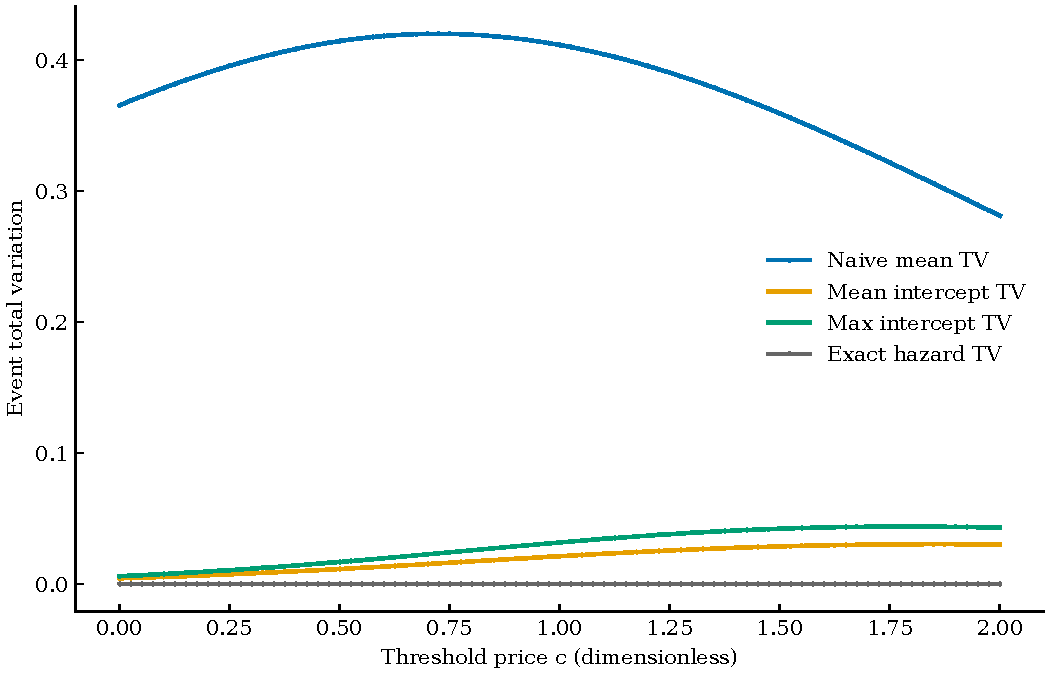
\includegraphics[width=0.70\textwidth]{figures/generated/slg-or-hazard-defect-20261111.pdf}\\[1ex]
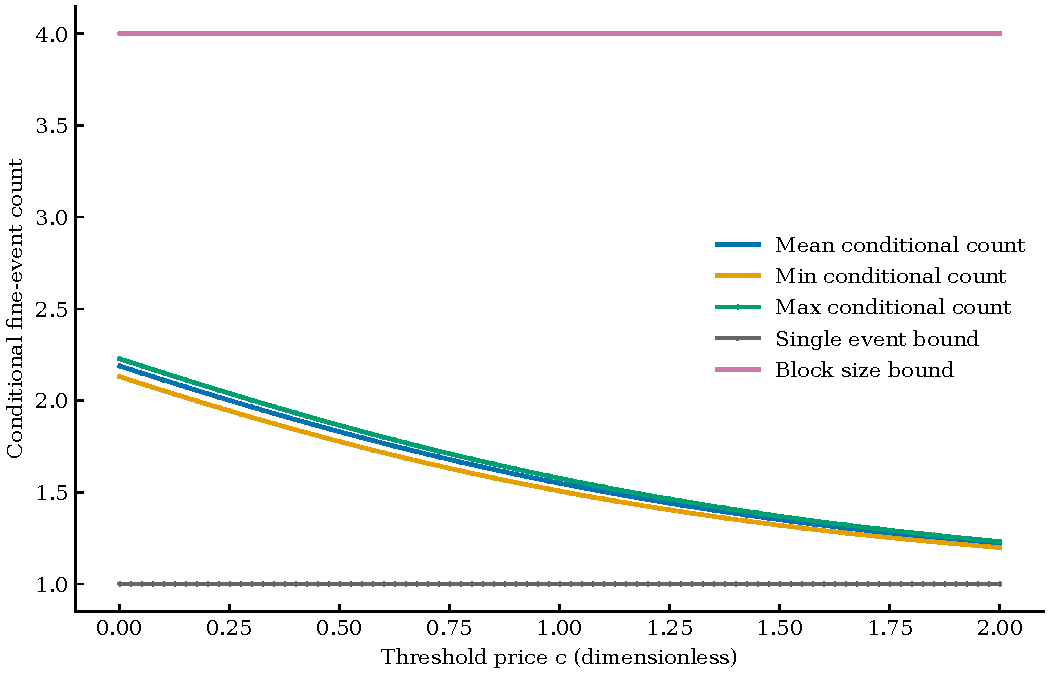
\includegraphics[width=0.70\textwidth]{figures/generated/slg-or-event-multiplicity-20261111.pdf}
\caption{Exact event closure and the cost of a smaller description. Top (a): Bernoulli event total variation over four externally frozen independent four-event schedules at 81 prices. Exact hazard retains \(h_B(c)\) and reproduces the OR probability. The naive law uses \(\sigma(S_B-c)\). The common-intercept law uses the arithmetic mean of block-specific \(c_{\mathrm{eff}}\) at each price. Its mean and maximum residuals quantify the effect of that restriction. The mean intercept minimises squared log-odds error, not TV. Bottom (b): for the same blocks, \(dc_{\mathrm{eff}}/dc=\mathbb E[N_B\mid N_B\geq1]\). Curves give its block mean, minimum and maximum, with exact bounds 1 and 4. This is conditional event multiplicity, not an instability eigenvalue. The full margin schedules are retained for repricing. A single hazard value at one price is insufficient for that response.}
\label{fig:num-toy-coarse-defect}
\end{figure*}

A slope above one therefore needs no critical or unstable mechanism. No iterated rescaled coupling transformation or fixed point has been defined here from which an RG eigenvalue could be extracted. Similarly, a negative effective intercept is an event log-odds offset produced by multiple opportunities, not negative physical work.

The dependence on price exposes another distinction. One number \(h_B(c_0)\) is sufficient for the OR probability at \(c_0\). It does not determine the entire function \(h_B(c)\), or even its derivative at \(c_0\). Repricing requires a richer retained description, such as the complete frozen margin schedule. Sufficiency is always relative to a question.

\subsection{Receiving dynamics requires more than event closure}
\label{subsec:receiving-dynamics}

For an actual adaptive learner, the current state and history determine the next margins. The appropriate object is its transition kernel or vector field, not an independent product law substituted along a realised trace. Exact aggregation of one event does not prove that a coarse state supports a closed adaptive process.

Let \(P(x,\cdot)\) be a finite-state fine Markov kernel, \(\pi:X\to Y\) a state map, and \(Q(y,\cdot)\) a proposed receiving kernel. Define total variation on their common receiving support by
\[
 \|\mu-\nu\|_{\mathrm{TV}}
       =\frac12\sum_{y\in Y}|\mu(y)-\nu(y)|.
\]
A one-step defect is
\begin{equation}
 \epsilon=
 \sup_{x\in X}
 \|\pi_*P(x,\cdot)-Q(\pi x,\cdot)\|_{\mathrm{TV}} .
 \label{eq:kernel-defect}
\end{equation}
Exact closure requires the pushed transition law to be identical for every fine state in a fibre. If initial coarse laws agree, the discrepancy after \(n\) steps is bounded by \(\min(1,n\epsilon)\). This bound uses TV contraction under a Markov kernel, not an assumption that the omitted variables cease to matter.

For smooth deterministic dynamics, let \(v\) be the fine field, \(w\) the receiving field, and \(\pi\) a differentiable map. The local mismatch is
\begin{equation}
 \delta(x)=\|D\pi_xv(x)-w(\pi x)\|.
 \label{eq:yba-app-infinitesimal-defect}
\end{equation}
The norm, domain and time window are part of the test. If \(\delta(x)\leq\delta_0\) along the trajectories and \(w\) is \(L\)-Lipschitz on a domain containing both compared paths, their initially equal coarse states remain within
\(\delta_0(e^{Lt}-1)/L\), with limit \(\delta_0t\) for \(L=0\). Appendix~\ref{app:maps} derives both receiving bounds.

Coordinate changes and coarse-graining should not be conflated. An invertible smooth coordinate map transports the complete field by the chain rule. A many-to-one map discards state. It can destroy autonomous dynamics even when all fine equations are correct. Restoring closure may require memory or another retained statistic rather than a different microscopic law. The OR calculation gives a concrete instance of finding the useful statistic instead of declaring every discrepancy a failure of learning.
